\tikzstyle{box} = [rectangle, minimum width=2.8cm, minimum height=0.7cm, text centered, draw=black]
\tikzstyle{arrow} = [thick,->,>=stealth]

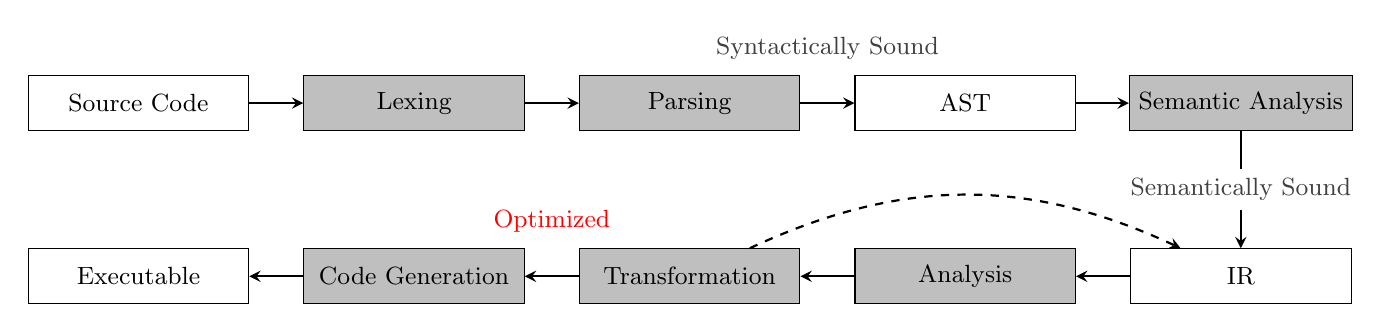
\begin{tikzpicture}
  \node (Source Code) [box] {\small Source Code};
  \node (Lexing) [box, fill=lightgray, right of=Source Code, xshift=2.5cm] {\small Lexing};
  \node (Parsing) [box, fill=lightgray, right of=Lexing, xshift=2.5cm] {\small Parsing};
  \node (AST) [box, right of = Parsing, xshift=2.5cm] {\small AST};
  \node (Semantic Analysis) [box, fill=lightgray, right of=AST, xshift=2.5cm] {\small Semantic Analysis};
  \node (Intermediate Representation) [box, below of=Semantic Analysis, yshift=-1.2cm, xshift=0cm] {\small IR};
  \node (Analysis) [box, fill=lightgray, left of=Intermediate Representation, xshift=-2.5cm] {\small Analysis};
  \node (Transformation) [box, fill=lightgray, left of=Analysis, xshift=-2.5cm] {\small Transformation};
  \node (Code Generation) [box, fill=lightgray, left of=Transformation, xshift=-2.5cm] {\small Code Generation};
  \node (Executable) [box, left of=Code Generation, xshift=-2.5cm] {\small Executable};

  \draw [arrow] (Source Code) -- (Lexing);
  \draw [arrow] (Lexing) -- (Parsing);
  \draw [arrow] (Parsing) -- node [fill=white, text=darkgray, yshift=0.7cm] {\small Syntactically Sound} (AST);
  \draw [arrow] (AST) -- (Semantic Analysis);
  \draw [arrow] (Semantic Analysis) -- node [fill=white, text=darkgray] {\small Semantically Sound} (Intermediate Representation);
  \draw [arrow] (Intermediate Representation) -- (Analysis);
  \draw [arrow] (Analysis) -- (Transformation);
  \draw [arrow, dashed] (Transformation) to [bend left=25] (Intermediate Representation);
  \draw [arrow] (Transformation) -- node [fill=white, text=red, yshift=0.7cm] {\small Optimized} (Code Generation);
  \draw [arrow] (Code Generation) -- (Executable);
\end{tikzpicture}